\section{Proton Absorption}

Because protons are strongly interacting particles, they may undergo a nuclear
reaction as they pass through the SHMS before forming an SHMS 3/4 trigger.
The corresponding electron in the HMS will have formed an HMS 3/4 trigger, but
the ``missing'' SHMS 3/4 will lead to a missing coincidence trigger.
As result, the total coincidence yield will be underestimated by some amount.
The proton absorption $A$ is the percentage of protons that, in this manner,
fail to form a coincidence trigger.


A theoretical estimate of the absorption can be obtained by considering the
proton's mean free path in the materials along its path through the SHMS.
Suppose a material is made up of components with atomic weights $A_i$, mass
density $\rho_i$, and total cross section $\sigma_{tot,i}$.
The nuclear collision length is
$\lambda_{T} = \sum_i A_i / (N_A \rho_i \sigma_{tot_i})$.
The nuclear interaction length $\lambda_{I}$ is similarly defined, subtracting
the elastic and quasielastic cross sections from $\sigma_{tot,i}$.
Because the elastic cross section is peaked in the forward direction, and will
thus remove few protons from the spectrometer's acceptance, we use the average
$\bar\lambda$ of $\lambda_T$ and $\lambda_I$ as our estimate of the mean free
path.
Our estimate of the absorption is $A=1-e^{-\sum_i X_i/\bar\lambda_i}$ where
$X_i$ is the thickness of each material in the proton's path.
Table~\ref{tab:shms_materials} lists the properties of relevant materials in
the SHMS.
Nuclear collision and interaction lengths are taken from
Ref~\cite{pdg_material_properties}.
Based on this table, we estimate the absorption to be $A=8.56\%$.


\vfill
% Note: in the multirow calls, the first argument is the height in lines I
% want the "system" name to span, not the number of rows in that section of
% the table.
\begin{table}[h]
    \centering
    \caption{Summary of materials in the SHMS that contribute to proton absorption.}
    \label{tab:shms_materials}
    \resizebox{1.0\textwidth}{!}{
        \begin{tabular}[t]{| l | l | l | r | r | r | r | r | r | r | r |}

            \hline
            System
            & Component                                       & Material & \thead{Thickness \\ (\si{cm})} & \thead{Density \\ (\si{\g\per\cubic\cm})} & \thead{X \\ (\si{\g\per\square\cm})} & \thead{$\lambda_T^{ a}$ \\ (\si{\g\per\square\cm})} & \thead{$\lambda_I^{ a}$ \\ (\si{\g\per\square\cm})} & \thead{$\bar{\lambda}$ \\ (\si{\g\per\square\cm})} & \thead{$X/\bar{\lambda}$ \\ ($10^-3$)}\\ \hline
            \hline

            \hline
            \multirow{6}{*}{\makecell[ml]{Target and \\ Magnets}}
            & LH2                                             & LH2                                   & 5.00                           & 0.07                                      & 0.35                                 & 42.80                                          & 52.00                                          & 47.40                                              & 7.38\\ \cline{2-10}
            & \makecell{Scattering chamber \\ exit window}    & Al                                    & 0.01                           & 2.7                                       & 0.03429                              & 69.70                                          & 107.20                                         & 88.45                                              & 0.39\\ \cline{2-10}
            & Air                                             & Air                                   & 30.00                          & 0.001                                     & 0.03675                              & 61.30                                          & 90.10                                          & 75.70                                              & 0.49\\ \cline{2-10}
            & HB entrance                                     & Al                                    & 0.03                           & 2.7                                       & 0.06858                              & 69.70                                          & 107.20                                         & 88.45                                              & 0.78\\ \cline{2-10}
            & Dipole exit                                     & Al                                    & 0.05                           & 2.7                                       & 0.13716                              & 69.70                                          & 107.20                                         & 88.45                                              & 1.55\\ \hline

            \hline
            \multirow{7}{*}{\makecell[ml]{Noble Gas \\ Cherenkov}}
            & \makecell{Entrance \\ window}                   & Tedlar                                & 0.01                           & 1.3                                       & 0.0066                               & 61.70                                          & 90.30                                          & 76.00                                              & 0.087\\ \cline{2-10}
            & Gas                                             & \makecell{\ch{CO2} \\ \SI{1.0}{\atm}} & 200.00                         & 0.002                                     & 0.396                                & 60.70                                          & 88.90                                          & 74.80                                              & 5.29\\ \cline{2-10}
            & Mirror                                          & \ch{SiO2}                             & 0.30                           & 2.2                                       & 0.66                                 & 65.20                                          & 97.80                                          & 81.50                                              & 8.10\\ \cline{2-10}
            & Mirror support                                  & Rohacell                              & 1.80                           & 0.11                                      & 0.198                                & -                                              & -                                              & 70.00                                              & 2.83\\ \cline{2-10}
            & Exit window                                     & Tedlar                                & 0.01                           & 1.3                                       & 0.0066                               & 61.70                                          & 90.30                                          & 76.00                                              & 0.087\\ \hline

            \hline
            \multirow{8}{*}{\makecell[ml]{Drift \\ Chambers}}
            & Entrance window                                 & Mylar                                 & 0.00254                        & 1.39                                      & 0.00353                              & 58.90                                          & 84.90                                          & 71.90                                              & 0.049\\ \cline{2-10}
            & Gas                                             & \makecell{50/50 \\ Ethane/Ar}         & 3.81                           & 0.002                                     & 0.00587                              & 68.60                                          & 101.00                                         & 84.80                                              & 0.069\\ \cline{2-10}
            & Field wire${^ b}$                               & W                                     & 0.00483                        & 2.7                                       & 0.01303                              & 69.80                                          & 108.00                                         & 88.90                                              & 0.147\\ \cline{2-10}
            & Sense wire${^ b}$                               & Be/Cu                                 & 0.00030                        & 19.3                                      & 0.00582                              & 110.00                                         & 185.00                                         & 147.50                                             & 0.040\\ \cline{2-10}
            & \makecell{Kapton in wire \\ and cathode planes} & Kapton                                & 0.18                           & 1.42                                      & 0.25248                              & 59.20                                          & 85.50                                          & 72.35                                              & 3.49\\ \cline{2-10}
            & Exit window                                     & Mylar                                 & 0.00254                        & 1.39                                      & 0.00353                              & 58.90                                          & 84.90                                          & 71.90                                              & 0.049\\ \hline

            \hline
            \multirow{2}{*}{\makecell[ml]{Hodoscope}}
            & \makecell{Scintilator \\ plane (x2.25)}         & PVT                                   & 1.13                           & 1.032                                     & 1.16100                              & 57.30                                          & 81.30                                          & 69.30                                              & 16.8\\ \hline

            \hline
            \multirow{5}{*}{\makecell[ml]{Heavy Gas \\ Cherenkov}}
            & Entrance window                                 & Al                                    & 0.10                           & 2.7                                       & 0.27                                 & 69.70                                          & 107.20                                         & 88.45                                              & 3.05\\ \cline{2-10}
            & Gas                                             & \makecell{\ch{CO2} \\ \SI{1.0}{\atm}} & 104.44                         & 0.002                                     & 0.20679                              & 60.70                                          & 88.90                                          & 74.80                                              & 2.76\\ \cline{2-10}
            & Mirror                                          & \ch{SiO2}                             & 0.30                           & 2.2                                       & 0.66                                 & 65.20                                          & 97.80                                          & 81.50                                              & 8.10\\ \cline{2-10}
            & Exit window                                     & Al                                    & 0.10                           & 2.7                                       & 0.27                                 & 69.70                                          & 107.20                                         & 88.45                                              & 3.05\\ \hline

            \hline
            \multirow{4}{*}{\makecell[ml]{Aerogel \\ Cherenkov}}
            & Entrance window                                 & Al                                    & 0.13                           & 2.699                                     & 0.35086                              & 69.70                                          & 107.20                                         & 88.45                                              & 3.97\\ \cline{2-10}
            & Aerogel                                         & Aeorogel                              & 9.00                           & 0.143                                     & 1.28571                              & 65.00                                          & 97.30                                          & 81.15                                              & 15.8\\ \cline{2-10}
            & Air                                             & Air                                   & 17.10                          & 0.001                                     & 0.02103                              & 61.30                                          & 90.10                                          & 75.70                                              & 0.28\\ \cline{2-10}
            & Exit window                                     & Al                                    & 0.16                           & 2.7                                       & 0.43200                              & 69.70                                          & 107.20                                         & 88.45                                              & 4.88\\ \hline
            \hline

            \hline
            \multirow{1}{*}{\makecell[ml]{Total}}
            &                                                 &                                       &                                &                                           &                                      &                                                &                                                &                                                    & 89.5\\ \hline

            \multicolumn{10}{l}{\multirow{1}{\linewidth}{\makecell[tl]{$^{a }$Nuclear
            interaction and collision lengths taken from
            PDG~\cite{pdg_material_properties}.}}} \\
            \multicolumn{10}{l}{\multirow{2}{\linewidth}{\makecell[tl]{$^{b }$The
            thicknesses of the wires are ``effective'' thicknesses, determined
            by the wire radii and cell spacings described \\ in
            subsection~\ref{subsec:drift_chambers}. This effective thickness
            of a single wire plane is the average thickness of a wire with
            radius r \\ repeated in a lattice of cell width w, seen by a particle whose position in the
            $XY$ plane is random. This effective \\ thickness is $\pi r^2/w$. \\}}}
        \end{tabular}
    } % resizebox
\end{table}
\vfill
\clearpage

\begin{figure}[!h]
    \centering
    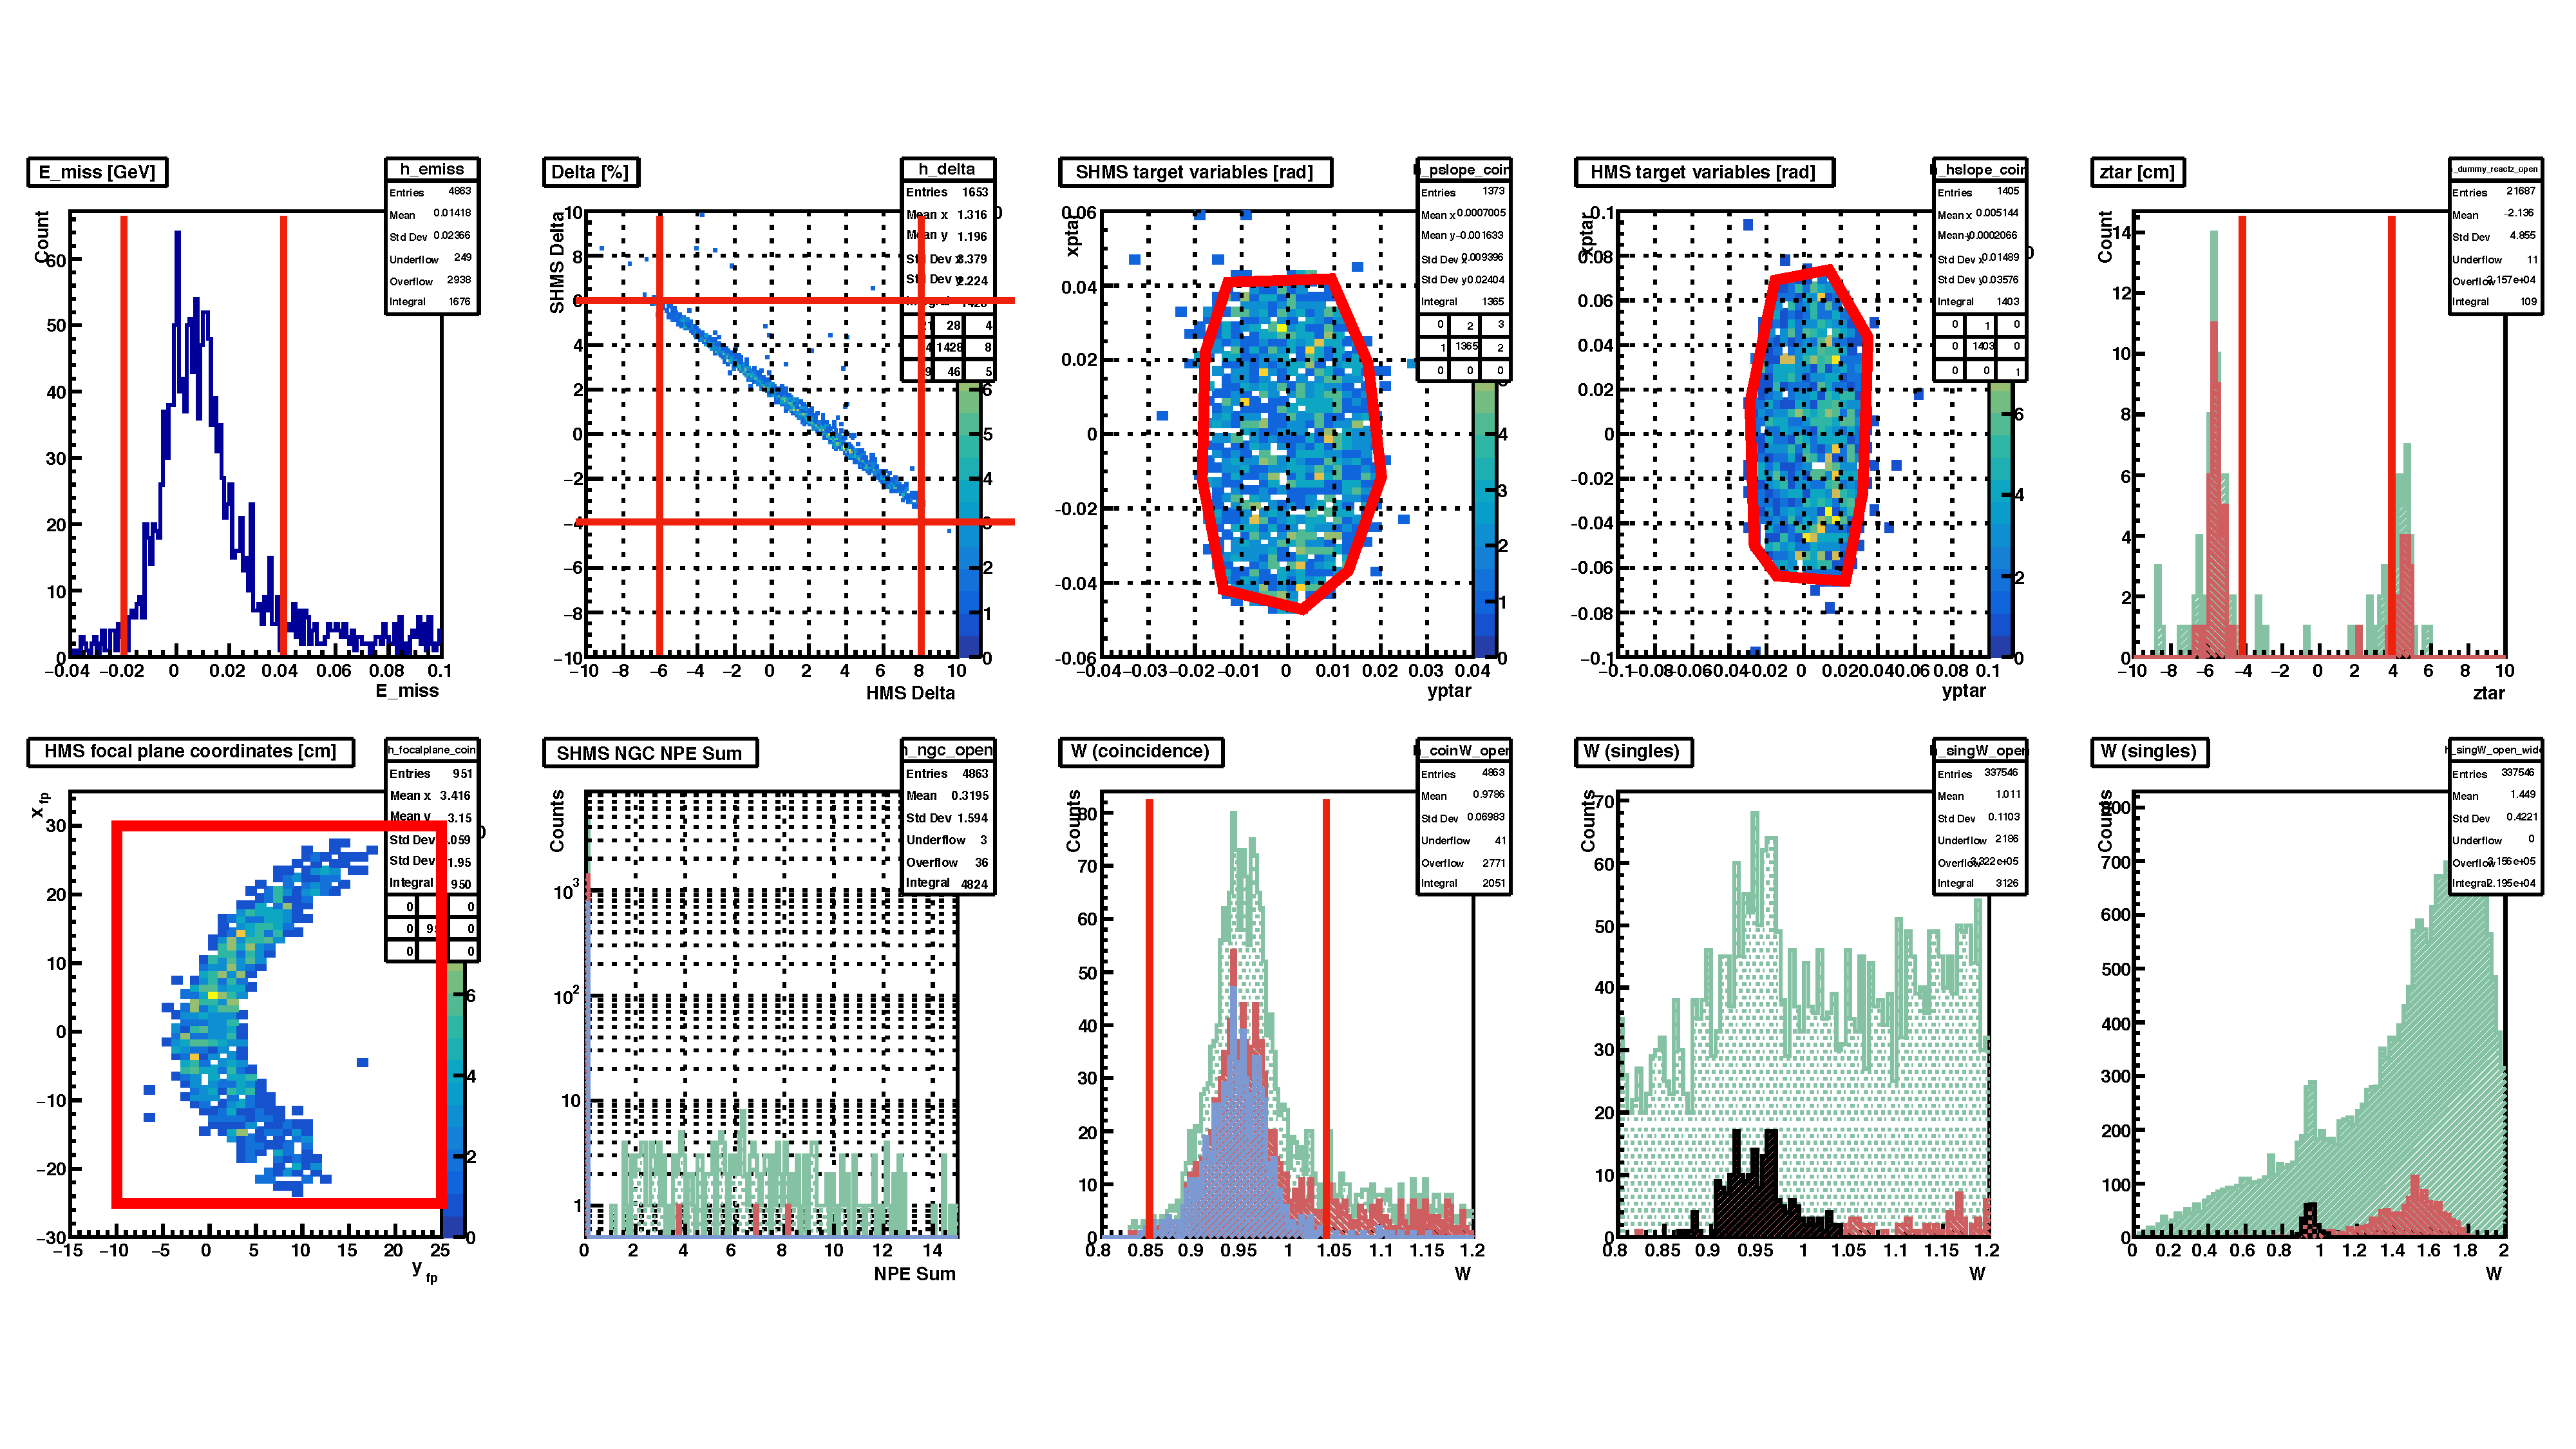
\includegraphics[width=1.0\textwidth]{chap4/proton_absorption_plots.pdf}
    \caption{Histograms of the quantities used to guide the selection of cuts
             for selecting H(e,e'p) events to estimate proton absorption.
             The red lines and contours indicate the cuts used.}
    \label{fig:proton_absorption_plots}
\end{figure}

Using the charge-normalized yields, $Y_{coin}$ and $Y_{sing}$, from coincidence
HMS singles H(e,e'p) runs, we can measure the proton absorption
$A=1-Y_{coin}/Y_{sing}$.
With a tight cut on spectrometer acceptance and invariant mass $W$ and
correcting for detector efficiencies and deadtime, $Y_{sing}$ should be an
accurate count of all electrons that participated in elastic scattering.
In contrast, $Y_{coin}$, even with the same cuts and corrections, will have
underestimated the ``true'' yield; some portion of the electrons detected in the
HMS will have corresponding protons that did not form a 3/4 trigger in the SHMS
because they were absorbed.
Using our $Q^2 = \SI{11.5}{\giga\electronvolt}$ runs and the cuts listed in
Table~\ref{tab:proton_absorption_cuts}, we estimate a proton absorption of $A=8.83 \pm 0.69 \%$.
The uncertainty quoted here is only statistical.

\begin{table}[h]
    \centering
    \caption{List of cuts used in proton absorption estimate.}
    \label{tab:proton_absorption_cuts}
    \resizebox{1.0\textwidth}{!}{
        \begin{tabular}[t]{| l | l |}
            \hline
            Variables              &  Cut \\ \hline
            \hline
            HMS PID                &  H.cer.npeSum>1 \&\& 0.90 < H.cal.etottracknorm \&\& H.cal.etottracknorm < 1.10 \\ \hline
            % ppidcut              &  P.ngcer.npeSum == 0 \\ \hline
            $E_{miss}$             &  -0.02 < P.kin.secondary.emiss \&\& P.kin.secondary.emiss<0.04 \\ \hline
            % pdeltacut            &  -4.0 < P.gtr.dp \&\& P.gtr.dp < 6.0 \\ \hline
            $\delta_{HMS}$         &  -6.0 < H.gtr.dp \&\& H.gtr.dp < 8.0 \\ \hline
            $x'_{tar}$,$y'_{tar}$  &  Graphical cut on HMS xptar and yptar shown in Figure~\ref{fig:proton_absorption_plots} \\ \hline
            % pslope               &  Graphical cut on SHMS xptar and yptar \\ \hline
            $z_{tar}$              &  abs(H.react.z)<3 \\ \hline
            $y_{tar}$              &  abs(H.gtr.y)<2 \\ \hline
            $x_{fp}$               &  -25<H.dc.x[0] \&\& H.dc.x[0]<30 \\ \hline
            $y_{fp}$               &  -10<H.dc.y[0] \&\& H.dc.y[0]<25 \\ \hline
            $W$                    &  0.85 < H.kin.W \&\& H.kin.W < 1.04 \\ \hline
        \end{tabular}
    } % resizebox
\end{table}

% TODO: list the method for choosing cuts
These cuts were selected by an iterative process of plotting a sequence of
histograms, each of which is plotted with a cut determined by the preceding
histograms in the sequence.
The relevant histograms are shown in Figure~\ref{fig:proton_absorption_plots}.
The process can be summarized as follows:
\begin{enumerate}
    \item Plot $E_{miss}$ for H(e,e'p) data using HMS Cherenkov and calorimeter cuts to select
        electrons. Select a cut around the peak of this distribution.
    \item Plot SHMS and HMS delta for H(e,e'p) data using that $E_{miss}$ cut and the HMS PID
        cuts. Select a cut on both.
    \item Plot HMS and SHMS $x'_{tar}$ vs $y'_{tar}$ for H(e,e'p) data using all prior cuts. Place
        a tight graphical cut on this distribution.
    \item Plot $z_{tar}$ and $y_{tar}$ for singles dummy data using cuts on HMS delta
        $x'_{tar}$, and $y'_{tar}$. Place cuts on $z_{tar}$ and $y_{tar}$ to
        remove events from the walls of the cell.
    \item Plot HMS $x_{fp}$ vs $y_{fp}$ for H(e,e'p) data using all prior cuts.
        Place a loose cut on this focal plane distribution.
    \item Define a subset of ``HMS-only'' cuts from the full set of cuts
        ``coincidence'' cuts selected so far.
    \item Examine the distributions of $W$ and SHMS Noble Gas Cherenkov NPE sum.
        Ensure that the HMS-only cuts are able to reproduce the $W$ distribution
        plotted using coincidence cuts. Ensure that there are not a significant
        number of pions showing up as non-zero entries in the SHMS Noble Gas
        Cherenkov NPE sum distribution.
    \item Using these HMS-only cuts, calculate the yields from coincidence and
        HMS singles H(e,e'p) data.
\end{enumerate}


\begin{figure}[!h]
    \centering
    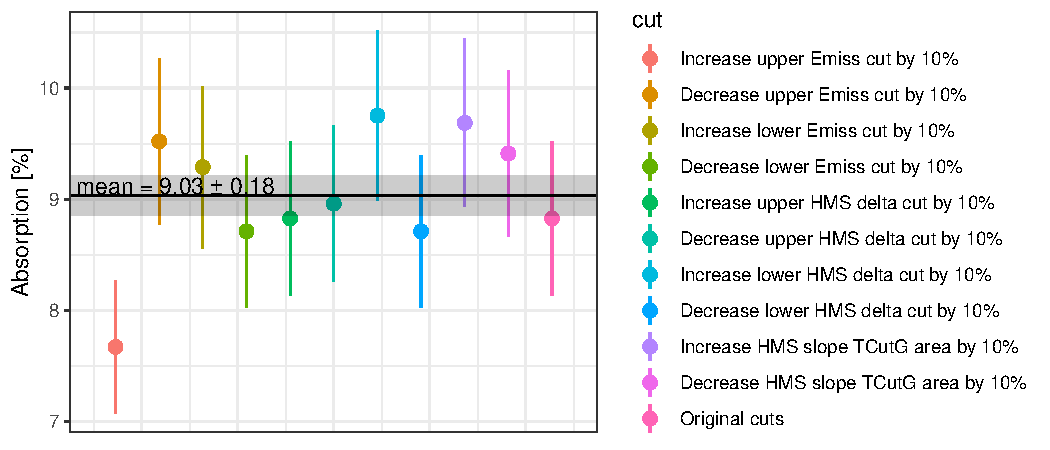
\includegraphics[width=1.0\textwidth]{chap4/proton_absorption_cut_study.pdf}
    \caption{Values of absorption estimated with 10\% variations on cuts used
             to select H(e,e'p) events.}
    \label{fig:proton_absorption_cut_study}
\end{figure}

To estimate the systematic uncertainty of this measurement, we varied the limits
of the following cuts by $\pm10\%$: $E_miss$, HMS delta, HMS xptar/yptar.
The absorption values for each of these variations are shown in
Figure~\ref{fig:proton_absorption_cut_study} along with the mean and standard
deviation of these estimates.
We use this value, $A=9.03\pm0.71\%$ as our final estimate of the proton
absorption, where the uncertainty is the quadrature sum of the systematic and
statistical uncertainties.
Note that the theoretical estimate of absorption is within the uncertainty in
this measurement.


While there are significant variations in proton-nucleus cross sections below
\SI{1}{\giga\electronvolt},
these cross sections reach plateaus around \SI{1}{\giga\electronvolt}
that have been measured up to the \si{\tera\electronvolt} range.
An incomplete catalog of hadron-nucleus cross section measurements can be found
in Refs~\cite{Carroll_1979, Kwong_1984, Denisov_1973, Ray_1979, Wellisch_1996,
Letaw_1983, Kohama_2016}.


Because these cross sections and thus the free path lengths are independent of
proton momentum over the range we studied (approximately 4 to
\SI{10}{\giga\electronvolt}), there is no momentum dependence in either our
estimate or measurement of proton absorption in the SHMS.
Therefore any uncertainty in proton absorption will only contribute to the
magnitude of measured transparencies, and not the presence or absence of a rise
in transparency with $Q^2$ characteristic of the onset of CT.

% TODO: list runs
% TODO: include a caveat about our poor statistics and a suggestion that this
%       measurement be duplicated in a future experiment?
% TODO: include reference to Carlos's HMS measurement
